\section{Spherical Harmonics}
\subsection{Property of Spherical Harmonics}
As mentioned in the previous section, the correlation method doesn't need to know individual orientation of diffraction pattern. It is very crucial to remove angle dependence of intensity since we want to recover particle structure. It is important that the selected function can be separated by its angle dependence and radius dependence. A set of functions that satisfies such criterion are spherical harmonics.

Spherical harmonics are a series of special function defined on the surface of sphere. It is defined in spherical coordinates represented by angles $\theta$ and $\phi$. The angular property of spherical harmonics is characterized by two quantum number namely $l$ and $m$. Another quantum number is $m$ represents how a function varies with respect to azimuthal angle. 

\begin{figure}[h]
  \centering
  \includegraphics[width=.8\textwidth]{sphexample}
\caption{Example of plot of spherical harmonics with different quantum numbers }
\label{fig:sphexample}
\end{figure}

The definition of spherical harmonics is given by
\begin{eqnarray}
Y_{lm}(\theta,\phi)=\sqrt{\frac{2l+1}{4 \pi}\frac{(l-m)!}{(l+m)!}} P_{lm}(\cos \theta) e^{im\phi}
\label{eq:sphhar}
\end{eqnarray}
where $P_{lm}(\cos \theta)$ is legendre polynomials. Legendre polynomial $P_{lm}(x)$ can be obtained using Rodrigues formula:
\begin{eqnarray}
P_{lm}(x)=\frac{(-1)^m}{2^{l} l!} (1-x^2)^{m/2}\frac{d^{l+m}}{dx^{l+m}}\left[(x^2-1)^l\right].
\label{eq:rodfor}
\end{eqnarray}

It is important to note that spherical harmonics are a polynomial of trigonometric function. As in other polynomial expansion, lower degree represents approximation of the function and higher degree contain information of how rapid the function varies.  

Since spherical harmonics are a set of functions characterized by 2 quantum numbers, it is important to show relation between those functions. Every single spherical harmonics function with different quantum number are orthogonal or mathematically it is represented by
\begin{eqnarray}
\int Y_{lm} Y_{l'm'}^{*} d\Omega= \delta_{ll'}\delta_{mm'}
\end{eqnarray}
where $\delta_{ll'}$ is Kronecker delta that is non zero only if indices are the same. 

The aim of this section is to characterize a symmetry in terms of spherical harmonic quantum numbers. In order to study rotational symmetry, an operator of rotation in spherical harmonics basis is needed. One well known operator to rotate spherical harmonics is the Wigner D-matrix. Definition below shows how spherical harmonics are rotated,
\begin{eqnarray}
Y_{lm}(\theta',\phi')=\sum_{m'}D^{l}_{mm'}(\alpha,\beta,\gamma)Y_{lm'}(\theta,\phi)
\end{eqnarray} 
where $\theta$, $\phi$ are with respect to original axes and the $\theta'$, $\phi'$ are with respect to rotated relative to their Euler angles ($\alpha$,$\beta$,$\gamma$). Elements of the Wigner D-matrix are calculated as follows:
\begin{eqnarray}
D^{l}_{mm'}(\alpha,\beta,\gamma)=e^{im'\gamma}d^{j}_{mm'}(\beta)e^{-im\alpha}
\end{eqnarray}
and $d^{j}_{mm'}$ is calculated by applying summation:
\begin{eqnarray}
&&d^{j}_{mm'}(\beta)=[(j+m')!(j-m)!(j+m)!(j-m)!]^{1/2}\\ \nonumber
&&\sum_{s}\frac{(-1)^{m'-m+s}}{(j+m-s)!s!(m'-m+s)!(j-m'-s)!} \cos(\frac{\beta}{2})^{2j+m-m'-2s} \sin(\frac{\beta}{2})^{m'-m+2s} ]
\end{eqnarray}

Another important property of spherical harmonics is they can be representated in a real basis function. It is easier to determine the number of the independent parameters in the real spherical harmonics because there is only the real number for all spherical harmonics expansion. A real basis of spherical harmonics is defined
\begin{align}
\begin{split}
Y_{lm}&=\sqrt(2)(-1)^{m} \operatorname{Im}(Y_{l|m|}) \quad \mbox{if} \quad m<0 \\
Y_{lm}&=Y_{l0} \quad \mbox{if} \quad m=0 \\
Y_{lm}&=\sqrt(2)(-1)^{m} \operatorname{Re}(Y_{l|m|}) \quad \mbox{if} \quad m>0. 
\end{split}
\label{eq:realsph}
\end{align} 

\subsection{Effect of Azimuthal Symmetry on Spherical Harmonics Expansion}
\label{subsec:azimsym}
It is very essential to discuss the azimuthal symmetry of the spherical harmonics. One important feature is how coordinate transformation affects the expansion of spherical harmonics. It will be shown here how by rotating coordinate and by setting z-axis as the center of symmetry, some component of spherical harmonics vanish.

In figure \ref{fig:azimuthrot}, the z-axis is not aligned to the center of symmetry of the object. Even though the object is a cylinder, which has azimuthal symmetry, none of spherical harmonics components will be zero. The reason is that by rotating the object with respect to z-axis the symmetry requirement is not satisfied. Having said that, rotation of axes is very important to determine  how symmetry of object affects spherical harmonics expansion.
 \begin{figure}[h]
  \centering
  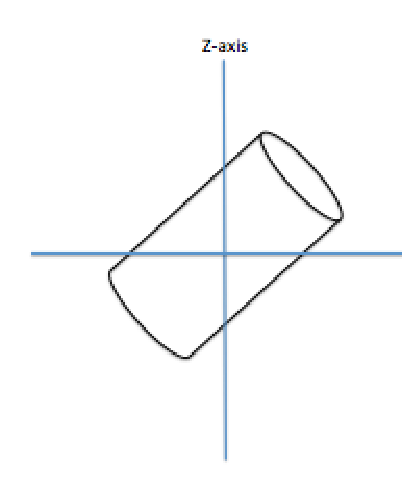
\includegraphics[width=.6\textwidth]{azimathrot}
\caption{Rotation of z-axis doesn't reveal azimuthal symmetry}
\label{fig:azimuthrot}
\end{figure}

In figure \ref{fig:azimuth}, the z-axis is now aligned to the center of symmetry of object. There is no change in appearance of object by rotation with respect to z-axis. Since symmetry is found in this coordinate transformation, there is pattern of m quantum number in spherical harmonics expansion.  
\begin{figure}[h]
  \centering
  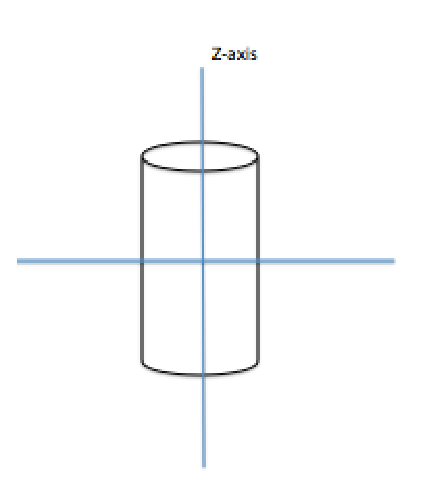
\includegraphics[width=.6\textwidth]{azimuth}
\caption{Rotation with respect to z-axis doesn't change the structure of object}
\label{fig:azimuth}
\end{figure}
By equating spherical harmonics before and after transformation,
\begin{eqnarray}
Y_{lm}(\theta,\phi)&=&Y_{lm}(\theta,\phi+\delta) \\ \nonumber
 Y_{lm}(\theta,\phi)&=&\sqrt{\frac{2l+1}{4 \pi}\frac{(l-m)!}{(l+m)!}} P_{lm}(\cos \theta) e^{im\left(\phi+\delta \right)} \\ \nonumber
\sqrt{\frac{2l+1}{4 \pi}\frac{(l-m)!}{(l+m)!}} P_{lm}(\cos \theta) e^{im\left(\phi \right)} &=& \sqrt{\frac{2l+1}{4 \pi}\frac{(l-m)!}{(l+m)!}} P_{lm}(\cos \theta) e^{im\left(\phi+\delta \right)} \\ \nonumber
e^{im\left(\phi\right)} &=& e^{im\left(\phi+\delta \right)}
\end{eqnarray}
$e^{im\left(\phi\right)} = e^{im\left(\phi+\delta \right)}$ is requirement to be satisfied if object has azimuthal symmetry with respect to z-axis. Since $\delta$ is any arbitrary angle, only $m=0$ satisfy the equation as it is shown in table \ref{tab:azim}
\begin{table}[h]
\begin{center}
  \begin{tabular}{ | c | c  |}
    \hline
    m & $e^{im\left(\phi\right)} = e^{im\left(\phi+\delta \right)}$  \\  \hline
    m=0 &\textcolor{red}{1=1} \\  \hline
    m=1 &$\cos( 1 \phi)+ i \sin(1 \phi) \neq \cos(1 (\phi+\delta))+ i \sin(1(\phi +\delta))$ \\  \hline 
    m=2 &$\cos( 2 \phi)+ i \sin(2 \phi) \neq \cos(2 (\phi+\delta))+ i \sin(2(\phi +\delta))$ \\  \hline 
    m=3 &$\cos( 3 \phi)+ i \sin(3 \phi) \neq \cos(3 (\phi+\delta))+ i \sin(3(\phi +\delta))$ \\  \hline 
    m=n &$\cos( n \phi)+ i \sin(n \phi) \neq \cos(n (\phi+\delta))+ i \sin(n(\phi +\delta))$ \\  \hline 
    \hline
  \end{tabular}
\end{center}
\captionof{table}{Only $m=0$ satisfy azimuthal symmetry since $\delta$ is arbitrary angle }
\label{tab:azim}
\end{table}
\begin{figure}[h]
  \centering
  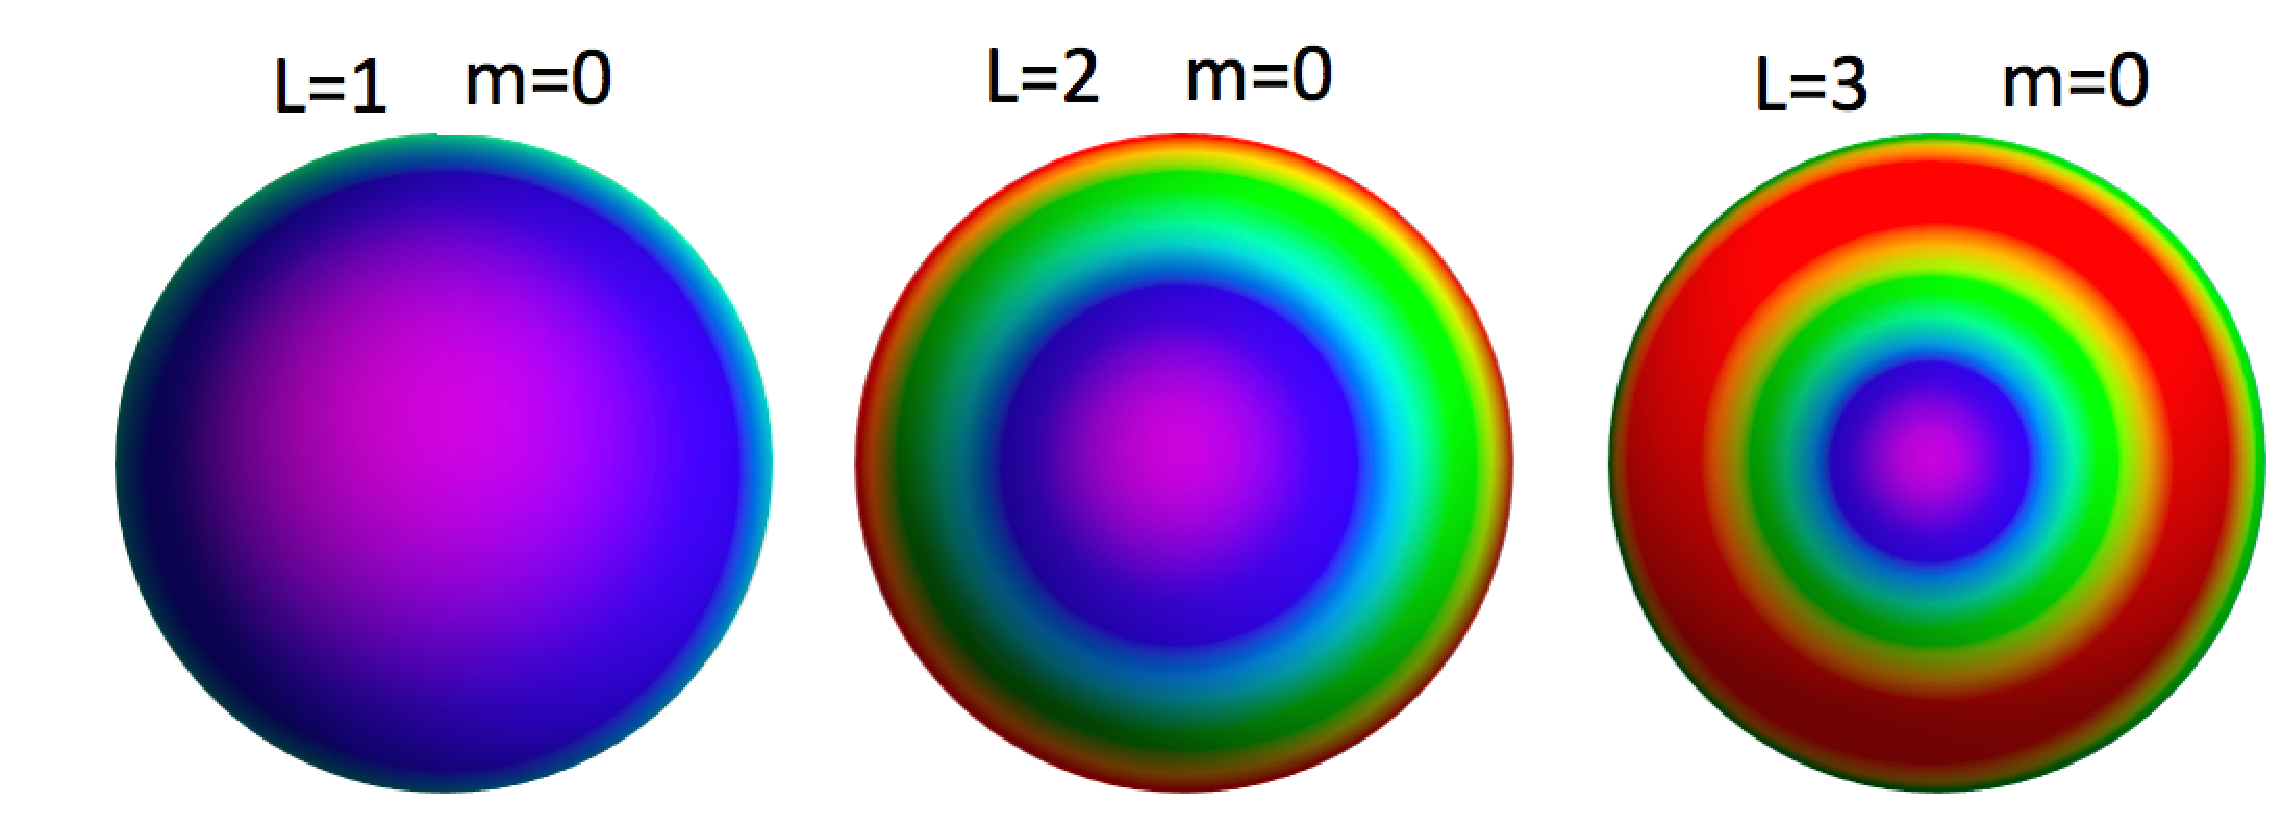
\includegraphics[width=.9\textwidth]{sphazm}
\caption{Plot of spherical harmonics with azimuthal symmetry}
\label{fig:sphazm}
\end{figure}
\subsection{Effect of 4-fold symmetry on Spherical Harmonics Expansion} \label{subsec:fold4}
The behavior of spherical harmonics that has 4-fold symmetry will be thoroughly explained here. The reason 4-fold symmetry is important is that later the object under study is a K-channel protein that satisfies 4-fold symmetry. Studying which expansion vanishes for given particular m quantum number enable one to determine if the object under study has 4-fold symmetry. 

As in the case of azimuthal symmetry, 4-fold symmetry is rotational symmetry with respect to z axis. The spherical harmonics axis can be arbitrary rotated, by setting the center of symmetry as z-axis, selection rule will appear as a result of the symmetry of the object.
\begin{figure}[h]
  \centering
  
\includegraphics[width=.6\textwidth]{4fold2}
\caption{Top view of object with 4-fold symmetry, rotation by $90^{0}$ doesn't change appearance of object }
\label{fig:4fold}
\end{figure}

Figure \ref{fig:4fold} is example of an object which has 4-fold symmetry and the center of symmetry is aligned with the z-axis. Rotation of angle $90^{0}$  or $\pi/2$ doesn't change structure of object. By equating spherical harmonics with the rotated one, one can find the quantum number that satisfy 4-fold symmetry. 
\begin{eqnarray}
Y_{lm}(\theta,\phi)&=&Y_{lm}(\theta,\phi+\frac{\pi}{2}) \\ \nonumber
 Y_{lm}(\theta,\phi)&=&\sqrt{\frac{2l+1}{4 \pi}\frac{(l-m)!}{(l+m)!}} P_{lm}(\cos \theta) e^{im\left(\phi+\pi/2 \right)} \\ \nonumber
\sqrt{\frac{2l+1}{4 \pi}\frac{(l-m)!}{(l+m)!}} P_{lm}(\cos \theta) e^{im\left(\phi \right)} &=& \sqrt{\frac{2l+1}{4 \pi}\frac{(l-m)!}{(l+m)!}} P_{lm}(\cos \theta) e^{im\left(\phi+\pi/2 \right)} \\ \nonumber
e^{im\left(\phi\right)} &=& e^{im\left(\phi+\pi/2 \right)}
\end{eqnarray}
$e^{im\left(\phi\right)} = e^{im\left(\phi+/pi/2 \right)}$ is the requirement to be satisfied if the object has 4-fold symmetry with respect to z-axis. Table \ref{tab:4fold} shows what quantum number persist if the object has 4-fold symmetry. 
\begin{table}[h]
\begin{center}
  \begin{tabular}{ | c | c  |}
    \hline
    m & $e^{im\left(\phi\right)} = e^{im\left(\phi+\pi/2 \right)}$  \\  \hline
    m=0 &\textcolor{red}{1=1} \\  \hline
    m=1 &$\cos( 1 \phi)+ i \sin(1 \phi) \neq \cos(1 (\phi+\pi/2))+ i \sin(1(\phi +\pi/2))$ \\  \hline 
    m=2 &$\cos( 2 \phi)+ i \sin(2 \phi) \neq \cos(2 (\phi+\pi/2))+ i \sin(2(\phi +\pi/2))$ \\  \hline 
    m=3 &$\cos( 3 \phi)+ i \sin(3 \phi) \neq \cos(3 (\phi+\pi/2))+ i \sin(3(\phi +\pi/2))$ \\  \hline 
    m=4 &\textcolor{red}{$\cos( 4 \phi)+ i \sin(4 \phi) = \cos(4 (\phi+\pi/2))+ i \sin(4(\phi +\pi/2))$} \\  \hline 
    m=5 &$\cos( 5 \phi)+ i \sin(5 \phi) \neq \cos(5 (\phi+\pi/2))+ i \sin(5(\phi +\pi/2))$ \\  \hline 
    m=6 &$\cos( 6 \phi)+ i \sin(6 \phi) \neq \cos(6 (\phi+\pi/2))+ i \sin(6(\phi +\pi/2))$ \\  \hline 
    m=7 &$\cos( 7 \phi)+ i \sin(7 \phi) \neq \cos(7 (\phi+\pi/2))+ i \sin(7(\phi +\pi/2))$ \\  \hline 
    m=8 &\textcolor{red}{$\cos( 8 \phi)+ i \sin(8 \phi) = \cos(8 (\phi+\pi/2))+ i \sin(8(\phi +\pi/2))$} \\  \hline 
    \hline
  \end{tabular}
\end{center}
\captionof{table}{Only $m=4n$, where n is integer, satisfy 4-fold symmetry }
\label{tab:4fold}
\end{table}
\begin{figure}[h]
  \centering
  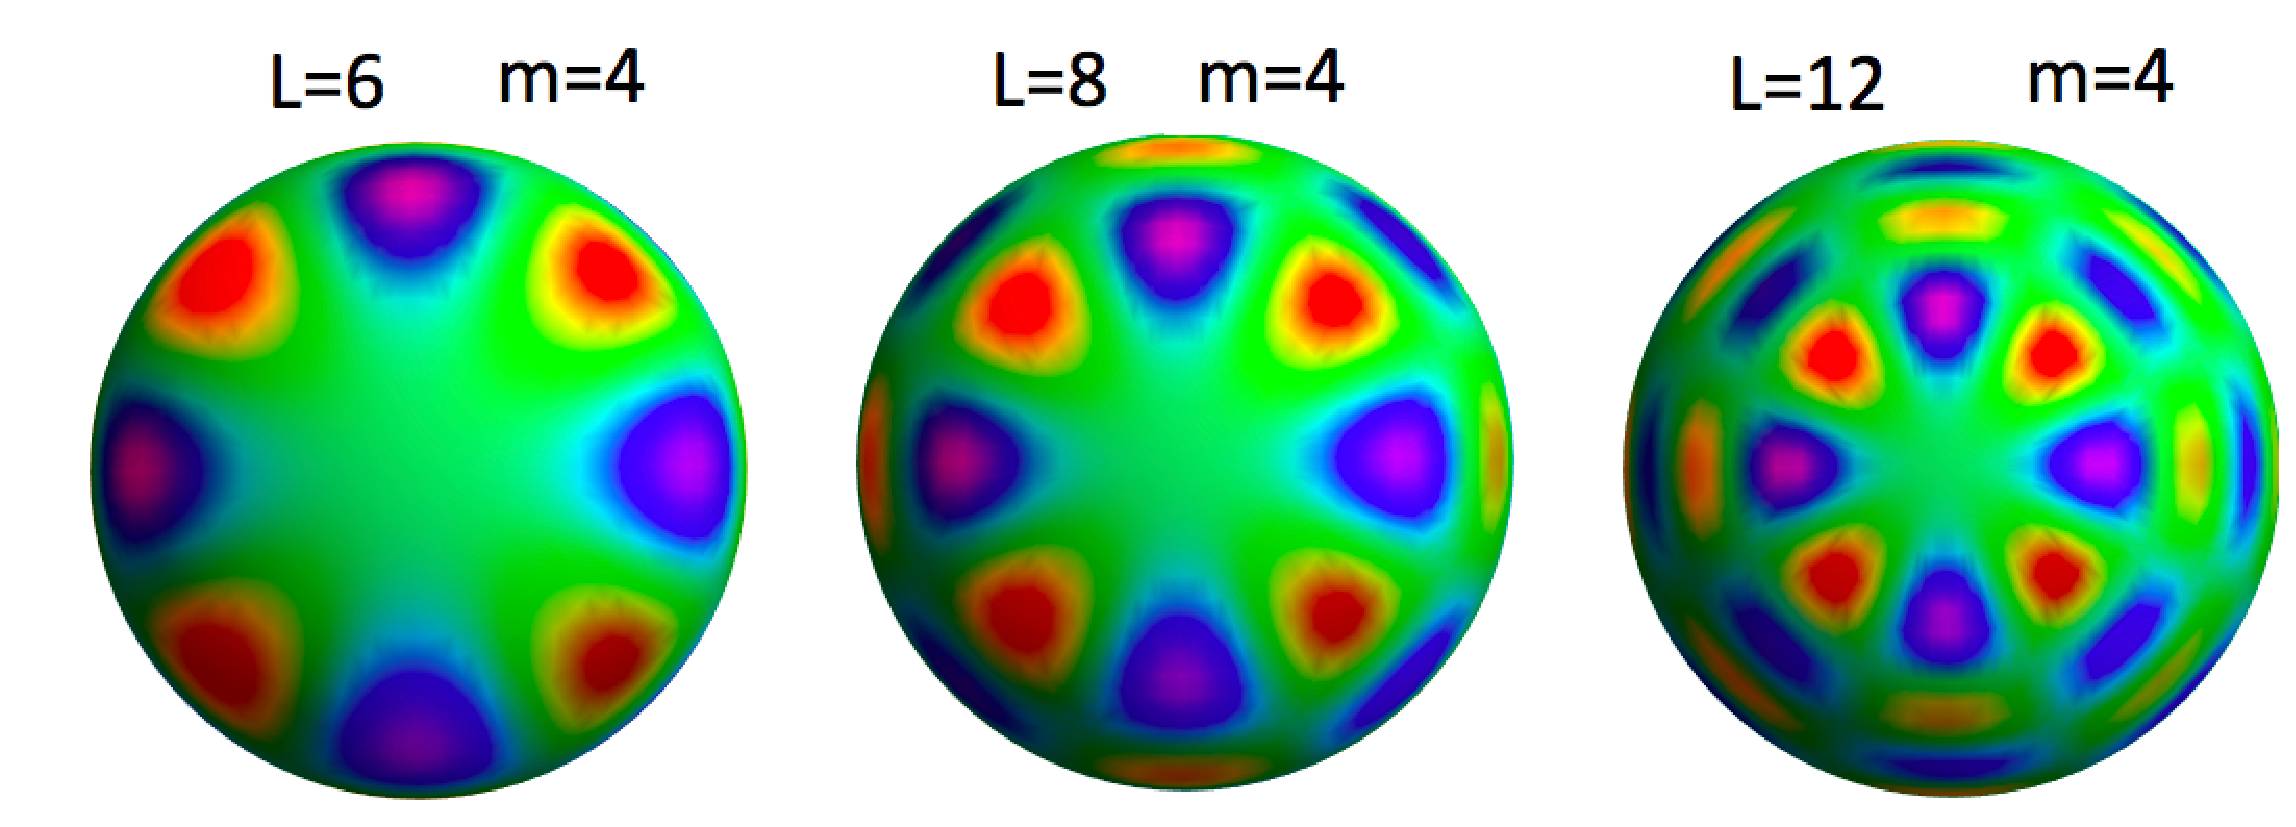
\includegraphics[width=.9\textwidth]{sph4fold}
\caption{Plot of spherical harmonics with 4-fold symmetry}
\label{fig:sph4fold}
\end{figure}
\subsection{Effect of Icosahedral symmetry on Spherical Harmonics Expansion} \label{icosph}
The behavior of spherical harmonics that has icosahedral symmetry will be thoroughly explained here. Previously, the symmetry under study is based on rotation of one axis only and the pattern involve only the $m$ quantum number. More complicated pattern will arise and quantum number in both $m$ and $l$ are necessary. One of symmetry which has more than one rotational axis is icosahedral symmetry. Studying which expansion vanishes for given particular m quantum number enable one to determine if the object under study has 4-fold symmetry.

Different than azimuthal and 4-fold symmetry, icosahedral symmetry has 3 rotational axes. They are 5-fold, 3-fold and 2-fold axes. The z-axis can be chosen arbitrary, by setting the center of symmetry as the 5-fold axis unique selection rule will appear as a result of the symmetry of the object. Based on icosahedral selection rule\cite{norahcohan}, $I_{lm}$ is nonzero when $l$ satisfy. 
\begin{eqnarray}
l=6p+10q \\
\text{where p and q in integer} \nonumber
\end{eqnarray}
and $m$ quantum numbers are
\begin{eqnarray}
m=...,-10,-5,0,5,10,...
\end{eqnarray}
when of 5-fold axis is taken as the z-axis. 
\begin{figure}[h]
  \centering
  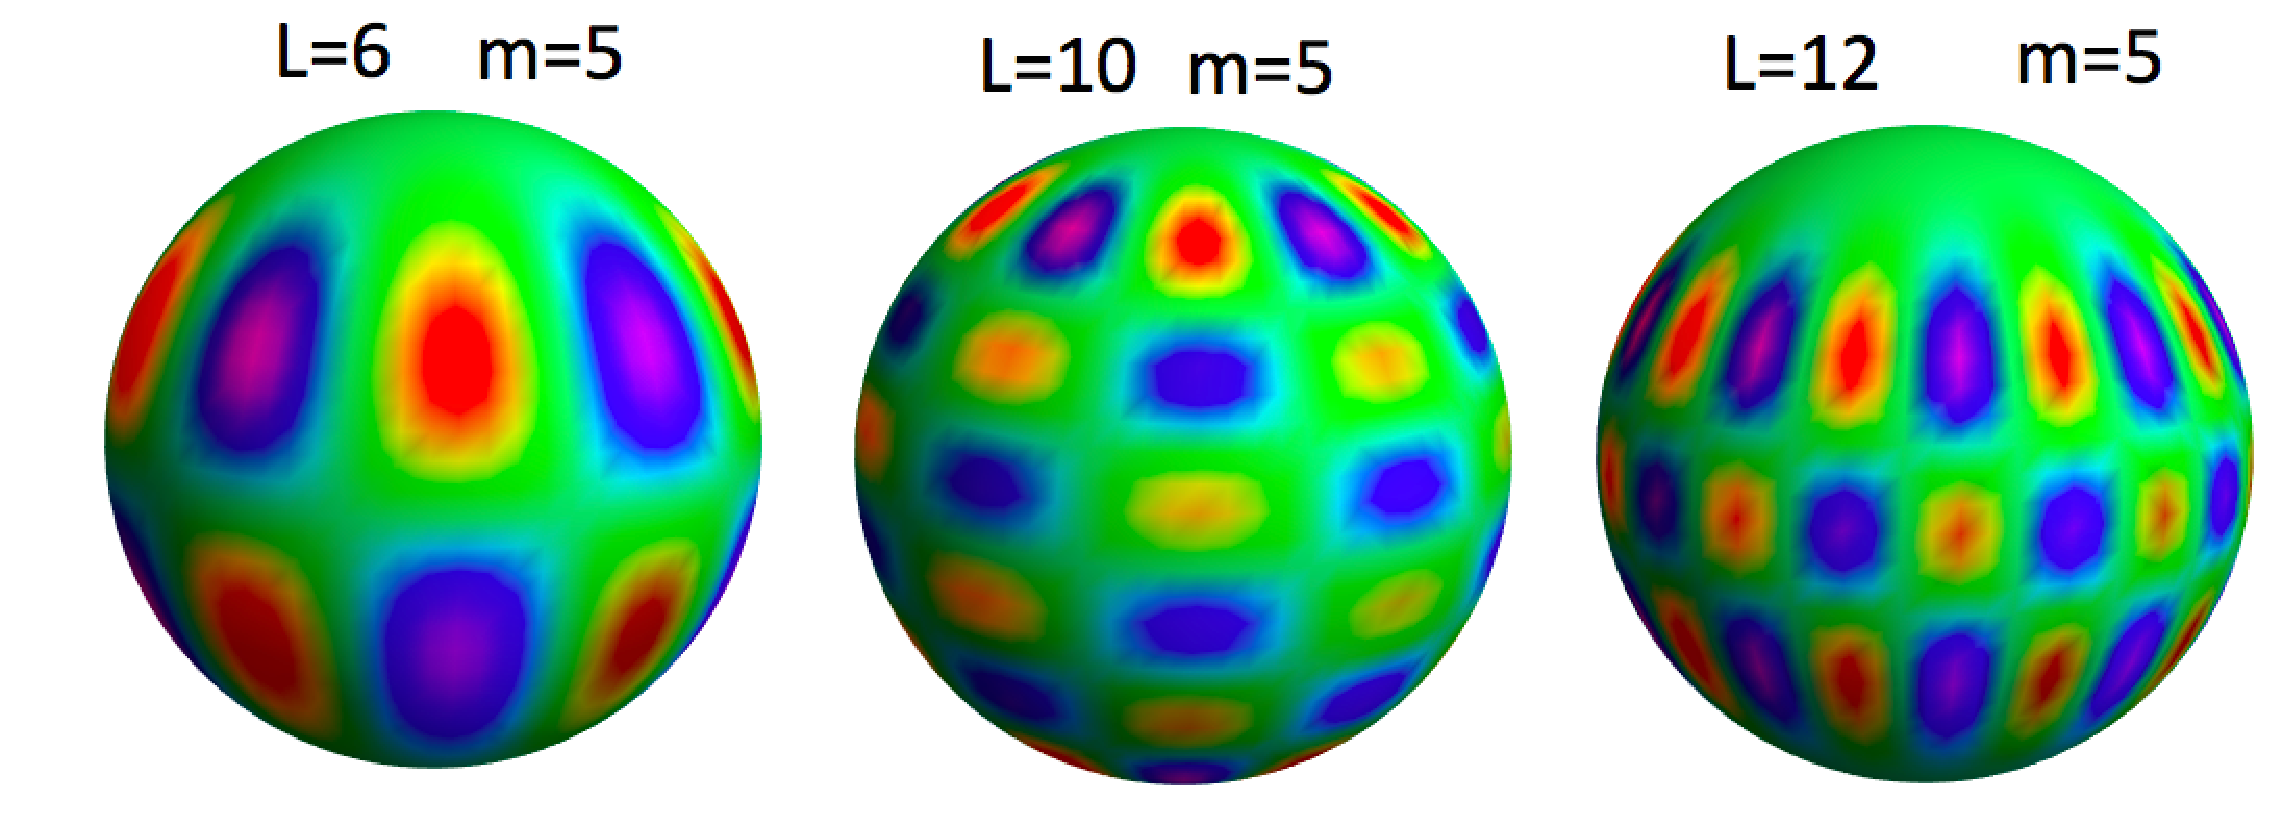
\includegraphics[width=.9\textwidth]{spico}
\caption{Plot of spherical harmonics with icosahedral symmetry}
\label{fig:icosymsph}
\end{figure}
A function can be constructed from a linear combination of spherical harmonics. In order to the function to satisfy icosahedral symmetry then only spherical harmonics which satisfies the selection rule are taken into the linear combination. In equation \ref{eq:icoharmonics}, $J_{l}(\theta,\phi)$ is an icosahedral harmonic which consist of a linear combination of spherical harmonics. By summing over all $m$, icosahedral harmonics only depend on $l$ quantum number.  

Factor $a_{lm}$ cannot be arbitrary because equation \ref{eq:icoharmonics} must satisfy icosahaderal symmetry\cite{harisonjack}. Table \ref{tab:spico} shows values of $a_{lm}$ for different combination of $l$ and $m$. Icosahedral harmonics are defined as linear combination of spherical harmonics which satisfy icosahedral symmetry:  
\begin{table}[h]
\begin{center}
  \begin{tabular}{ | c | c  | c | c | c | c |}
    \hline
    l\ m & 0 & 5 & 10 & 15 & 20  \\  \hline
    0 & 1.0 & & & &  \\  \hline
    6 & 0.531085 & 0.847318 & & & \\  \hline 
    10 &0.265539 &-0.846143 &0.462094 & & \\  \hline 
    12 &0.454749 &0.469992 &0.75613 & & \\  \hline 
    16 &0.334300 &-0.493693 &-0.634406 &0.491975 &\\  \hline 
    18 &0.399497 &0.450611 &0.360958 &0.712083 &\\  \hline 
    20 &0.077539 &-0.460748 &0.747888 &-0.231074 &0.411056\\  \hline 
    \hline
  \end{tabular}
\end{center}
\captionof{table}{Coefficient of spherical harmonics to convert into icosahedral harmonics \cite{saldinvirus} }
\label{tab:spico}
\end{table}
\begin{eqnarray}
J_{l}(\theta,\phi)=\sum_{m} a_{lm} Y_{lm}(\theta,\phi)
\label{eq:icoharmonics}
\end{eqnarray}
From table \ref{tab:spico}, $I_{lm}$ is nonzero if $m$ is a multiple 5. By looking at equation \ref{eq:icoharmonics}, for a particular $l$, $I_{lm}$ is not independent if the object has icosahedral symmetry. The spherical harmonics expansion of an icosahedral object only depends on values of $l$, given the $l$ the values of $m$ are determined by symmetry and are tabulated. In other words, for icosahedral object there is one independent parameter for each $I_{lm}$.

